\documentclass[10pt]{article}
\fontfamily{times}
\usepackage[utf8]{inputenc}
\usepackage{graphicx}
\setlength{\parindent}{0pt}
\setlength{\parskip}{1ex}
\usepackage{amsmath,amsfonts,amsthm}
\DeclareMathOperator{\E}{E}
%\textwidth=15cm
\usepackage[super,comma]{natbib}
\bibliographystyle{vancouver2}
% \bibliographystyle{unsrtnat}

\makeatletter \renewcommand\@biblabel[1]{#1} \makeatother

\begin{document}

\begin{center}
{\large \bf  Efficient Prevalence Estimation and Population Screening\\ for SARS-CoV-2\\\vspace*{0.5cm} Supplementary Material  }                           
\end{center}

Kenneth Gundersen, Jan Terje Kvaløy, Håkon K. Gjessing and Iren Løhr

\vspace*{10mm}

This supplementary file first provides the plots referenced in the main text. The calculations behind the plots are explained at the end of the document. The R code used to generate the plots can be found in the GitHub repository: xxxxxx    

\subsubsection*{Prevalence estimation}

Figure~\ref{S1} shows 90\% confidence intervals for the estimated prevalence obtained for different sample sizes (number of persons sampled), degrees of pooling, and prevalences. Figure~\ref{S3} below shows the sensitivity assumed in these calculations, depending on the degree of pooling.
 
\begin{figure}[!hbt]
\begin{center}
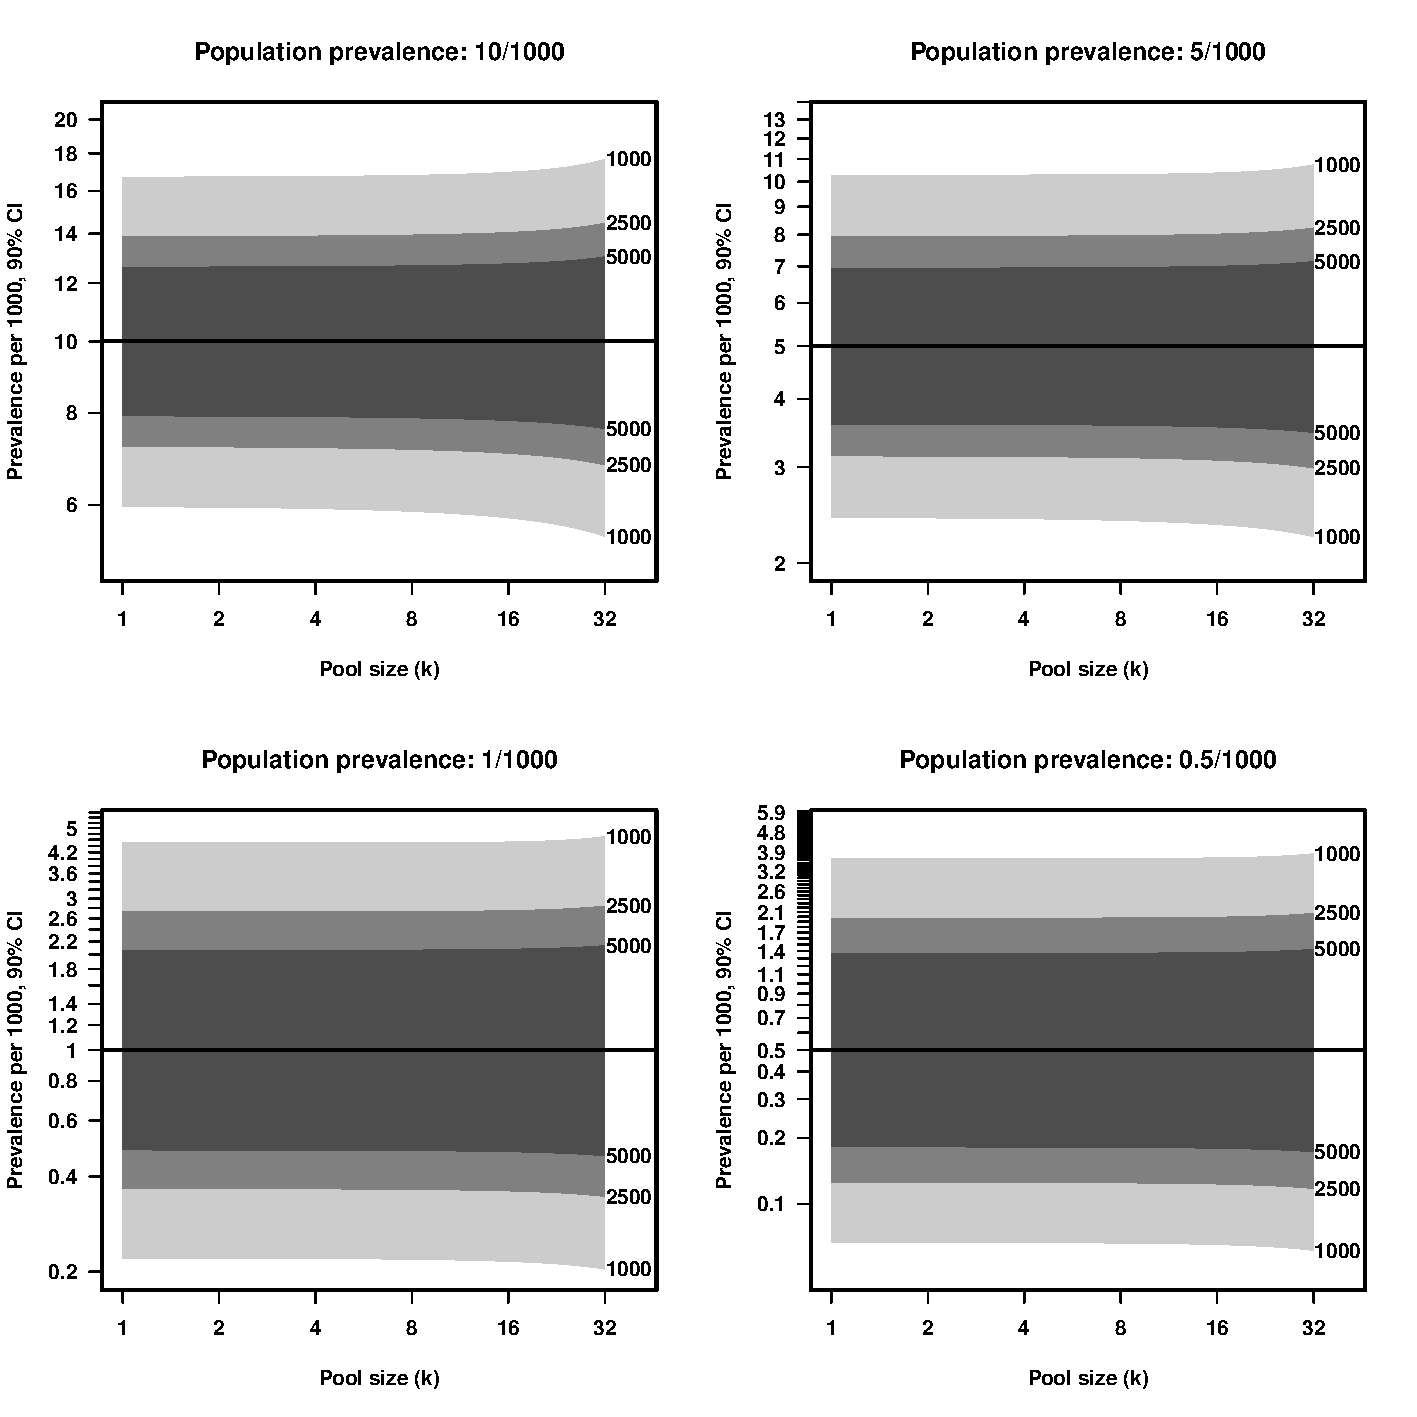
\includegraphics[width=0.95\linewidth]{prevalences_CI.pdf}
\end{center}
\caption{Precision (90\% confidence intervals) of prevalence estimates based on pooled sampling, depending on prevalence, degree of pooling, and the total number of persons sampled (shown in right hand column of the plot). Note that the number of pools needed to be analyzed is the number of persons divided by the degree of pooling. The calculations assume a pool analysis sensitivity as shown in Figure~\ref{S3}. See text for further description.}
\label{S1}
\end{figure}

\subsubsection*{Screening}

Figure~\ref{S2} shows how many persons can be included in the screening and the expected number of infected persons identified for three different screening strategies. The first strategy is to do no pooling. The second strategy is to first test samples in pools of 8. For the pools that are positive, samples from all 8 persons are tested individually. In the third strategy samples are first tested in pools of 32. For pools that are positive a second test in 4 pools of size 8 are made. Then finally for the positive pools of 8, individual tests are run. 

\begin{figure}[!hbt]
\begin{center}
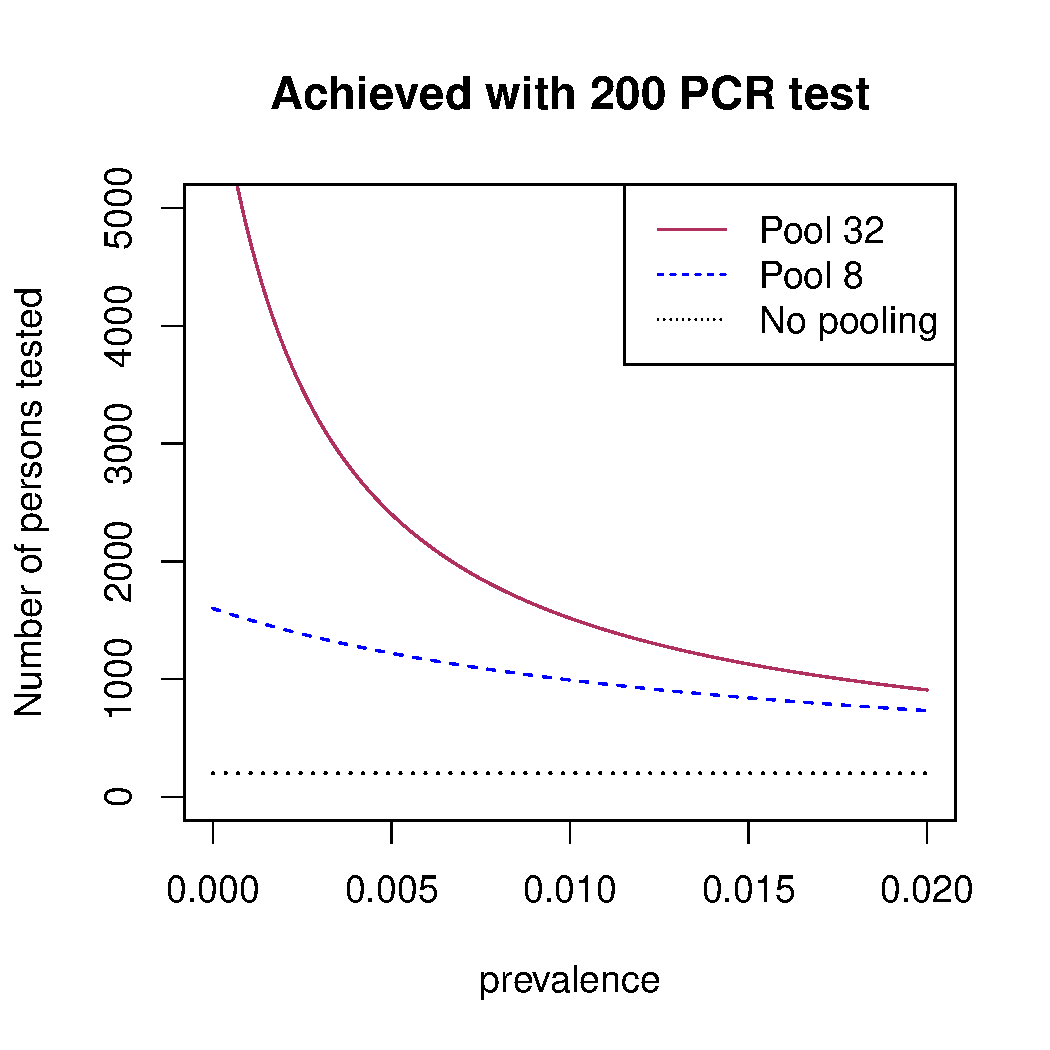
\includegraphics[width=0.48\linewidth]{ntested200.pdf}
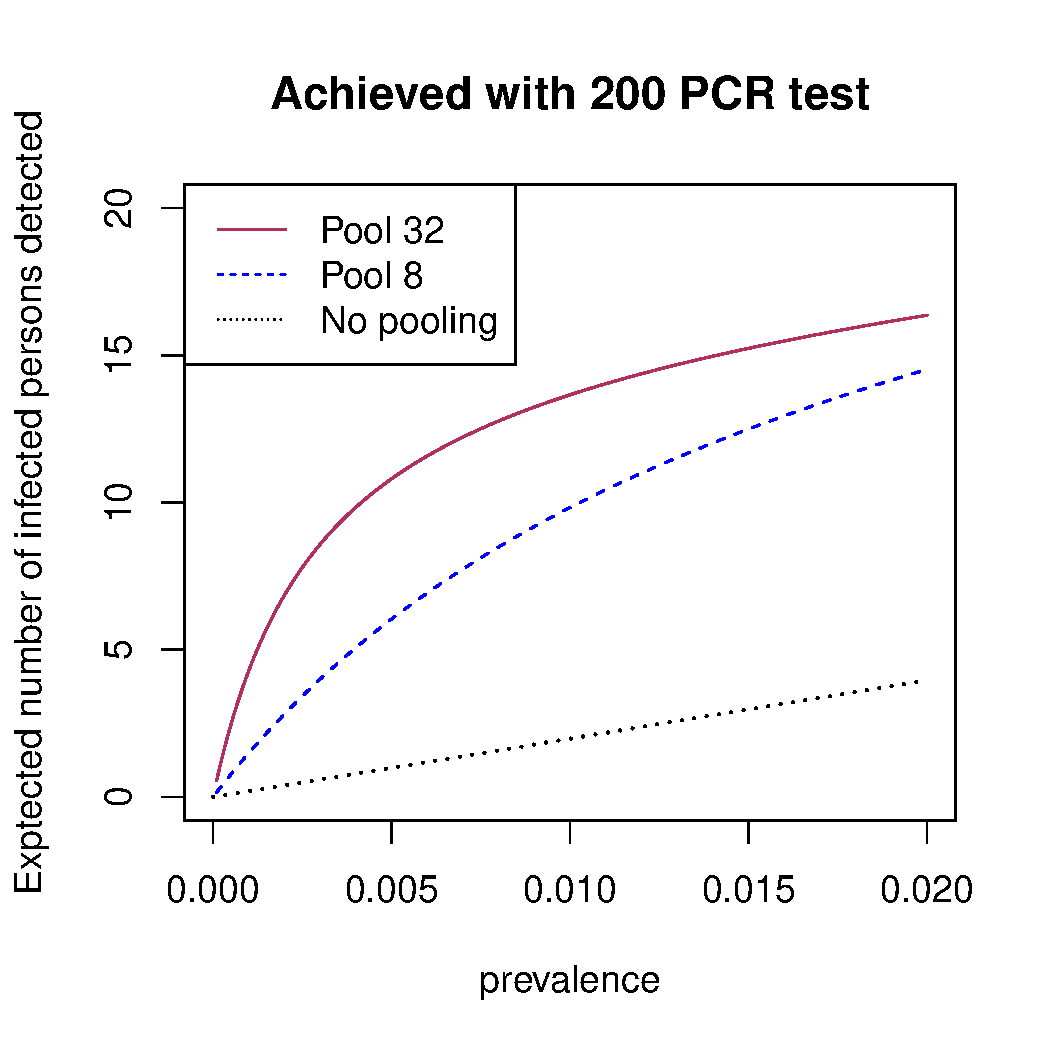
\includegraphics[width=0.48\linewidth]{ndetected200.pdf}\\
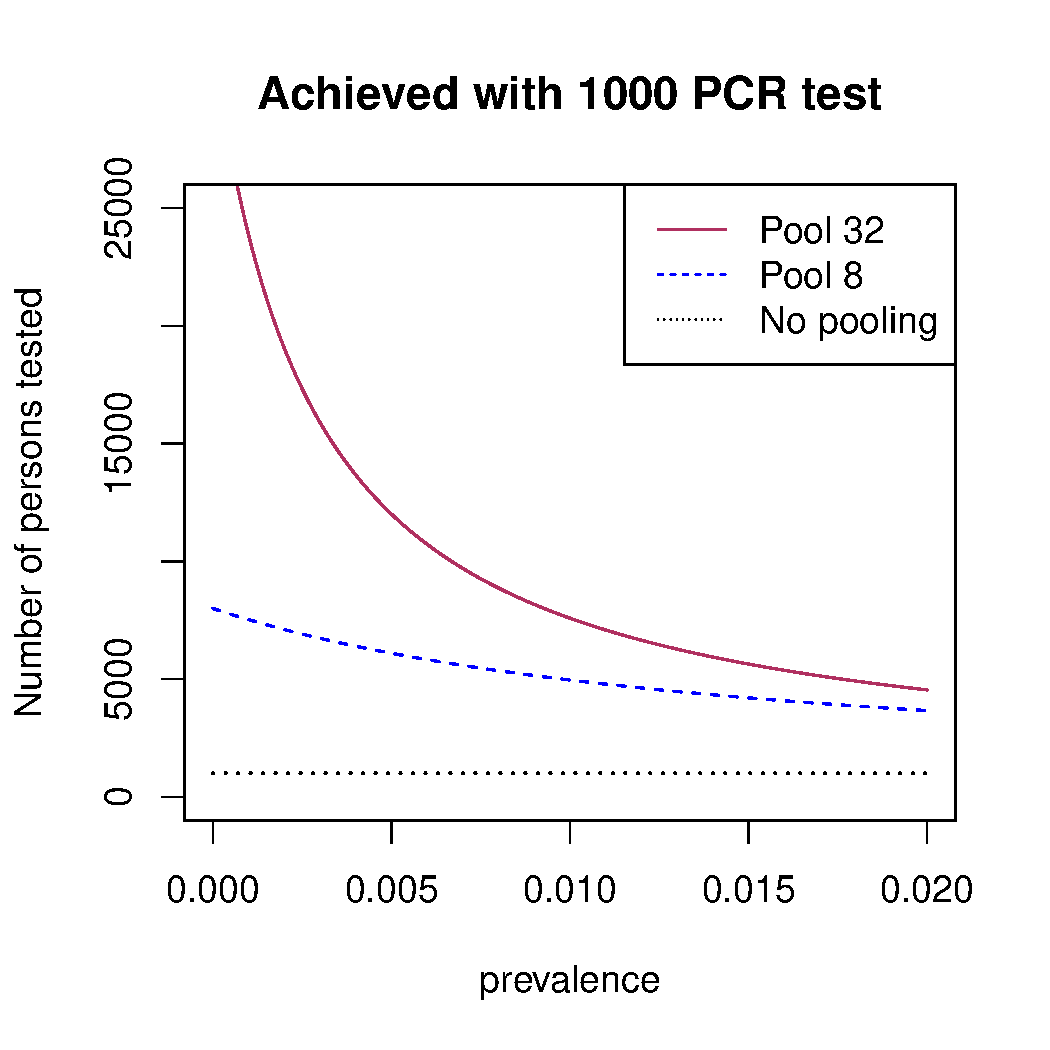
\includegraphics[width=0.48\linewidth]{ntested1000.pdf}
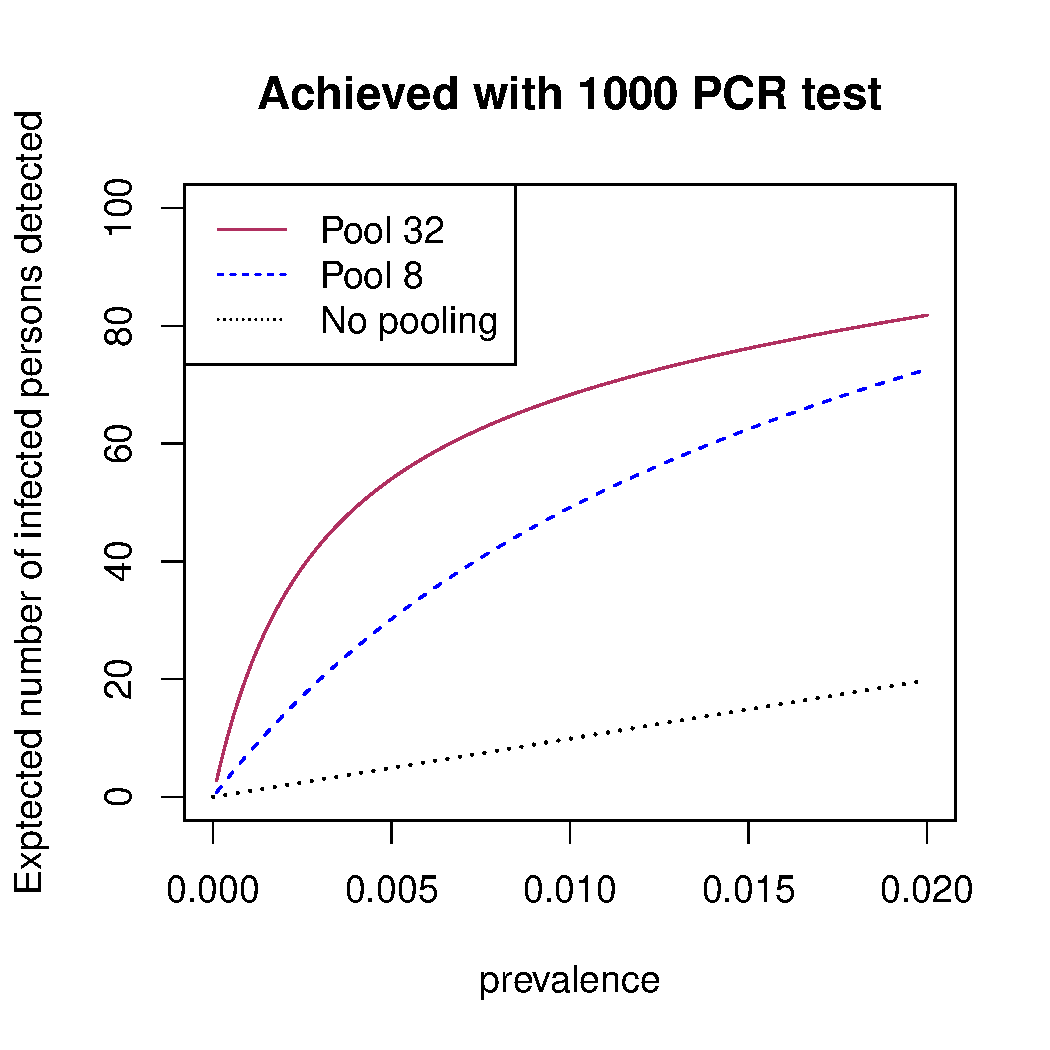
\includegraphics[width=0.48\linewidth]{ndetected1000.pdf}\\
\end{center}
\caption{The left plots depicts the number of persons that could be tested and the right plots the expected number of infected persons that would be identified with two different PCR budgets and three different test strategies: 1) No pooling; 2) Pool size 8 in the first testing and re-testing of all samples in the positive pools; 3) Pool size 32 in the first testing, re-testing in pools of 8 for the positive pools, re-testing all for the positive pools of size 8.}
\label{S2}
\end{figure}


In the illustrations shown in Figure~\ref{S2}  we have assumed a sensitivity of 99\% for pools of size 8 and a sensitivity of 90\% for pools of size 32.  Similar plots for other scenarios can be generated using the R code in the GitHub repository. Note that both the numbers of persons included and the expected number of cases identified scale linearly with the number of available PCR analyses. For 1000 analyses the numbers are five times that of 200 analyses.

\subsubsection*{Mathematical details}

Let $p$ be the true prevalence, $k$ the number of samples merged in one pool and $\pi(k)$ the probability that a pool of $k$ tests is positive. Let further $s(k)$ be the sensitivity of the test for a pool of  $k$ tests. Then
\begin{equation}
\label{pip}
\pi(k)=s(k)(1-(1-p)^k).
\end{equation}
\paragraph*{Prevalence estimation}
For prevalence estimation, $p$,  we first  estimate $\pi(k)$ by 
\begin{equation}
\label{pihat}
\hat{\pi}(k)=\frac{N_{+}}{N}
\end{equation}
where $N_{+}$  is the number of positive pools and $N$ is the number of pools.  The total number of persons tested is $n_{pers}=kN$. From (\ref{pip})  and (\ref{pihat}) we get that 
\begin{equation}
\label{phat}
\hat{p}=1-\left(1-\frac{\hat{\pi}(k)}{s(k)}\right)^{1/k}=1-\left(1-\frac{N_+}{s(k)N}\right)^{1/k}.
\end{equation}
\begin{figure}[!hbt]
\begin{center}
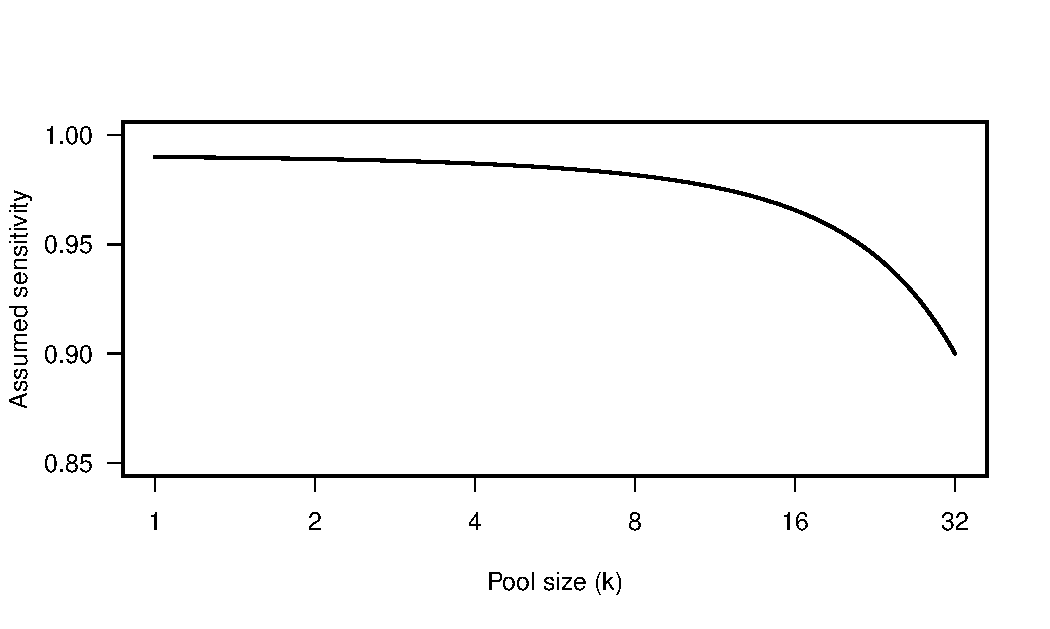
\includegraphics[width=0.85\linewidth]{sens_assumed.pdf}
\end{center}
\caption{Sensitivity of pooled samples, as assumed in the confidence interval calculations for Figure~\ref{S1}}
\label{S3}
\end{figure}
Moreover, to obtain a confidence interval for $\hat p$ we propose to first calculate Wilson confidence intervals \cite{agresti_approximate_1998} for $\hat{\pi}(k)$ and map this to confidence limits for $\hat p$ by inserting the upper and lower limits in (\ref{phat}). Wilson confidence intervals are available from the {\tt binom.confint} function in the {\tt R} package {\tt binom} \cite{R,binom}. Additional statistical tools for computing prevalences from pooled samples can be found in the {\tt prevalence} package \cite{prevalence,speybroeck_estimating_2012}.

\paragraph*{Screening strategies}
For considerations around the screening strategies let first $N_{PCR}$ be the total number of PCR analyses which needs to be performed and let $N_{PCR,1}$ be the number of PCR analyses run in the first round. With no pooling $N_{PCR}=N_{PCR,1}$. For pooling stratgies $N_{PCR}$ will be a random variable since we do not know how many positive pools we will find. For the strategy with pooling of 8 samples we have
$$
\E(N_{PCR})=N_{PCR,1}+N_{PCR,1}\cdot\pi(8) 8 
\;\;\;\;  \Rightarrow  \;\;\;\;
N_{PCR,1}=\frac{\E(N_{PCR})}{1+\pi(8) 8}. 
$$
By inserting the budget of available PCR analyses for $\E(N_{PCR})$ (e.g. 200 and 1000 in Figure~\ref{S2}) we get that the total number of persons that can be tested is $n_{pers}=8N_{PCR,1}$. Let $n_{pos}$ be the total number of identified positive cases, and let $n_{pos,8}$ denote the number of positive cases in a pool of 8. Then
$$
\E(n_{pos})=N_{PCR,1}\cdot\pi(8)\E(n_{pos,8}|n_{pos,8}\geq 1)=\frac{N_{PCR,1}\cdot \pi(8) 8 p}{(1-p)^8}.
$$  

For the strategy starting with 32 pools then re-testing in pools of 8 if positive and finally testing all samples in positive pools of 8, similar calculations give. 
$$
N_{PCR,1}=\frac{\E(N_{PCR})}{1+\pi(32) (4+8 \E(X|n_{pos,32}\geq 1))}.  
$$
Here $X$ is the number of positive pools among four pools of size 8, and $\E(X|n_{pos,32}\geq 1)$ can be approximated by
\begin{eqnarray*}
\E(X|n_{pos,32}\geq 1) &=& [P(n_{pos,32}=1)+(\frac{7}{31}+2\frac{24}{31})P(n_{pos,32}=2)  \\
&& +(\frac{7}{31}\frac{6}{30}+2(\frac{7}{31}\frac{24}{30}+\frac{24}{31}\frac{14}{30})+3\frac{24}{31}\frac{16}{30})P(n_{pos,32}=3)\\
&& +4P(n_{pos,32}\geq 4) ]/P(n_{pos,32}\geq 1).
\end{eqnarray*}
The last term $4P(n_{pos,32}\geq 4)$ implies that this is an upper bound, the approximation being very accurate for small $p$. Finally, we get the expected number of detections by
$$
\E(n_{pos})=N_{PCR,1}\cdot\pi(32)\E(n_{pos,32}|n_{pos,32}\geq 1)=\frac{N_{PCR,1}\cdot \pi(32) 32 p}{(1-p)^{32}}.
$$  
\section*{Acknowledgements}
We thank Ola Brønstad Brynildsrud for useful discussions.
\bibliography{refs}{}


\end{document}
